% Author: Carles Marin (Claude, Anthropic, as AI research assistant).
% Version en espanol de "Anomaly- and Tadpole-Compatible Fermion Completion of 6D SU(4) GHU".
% Narrativa guiada por preguntas; fisica primero, metodo exacto en apoyo. Build: pdflatex x2.
\documentclass[11pt,a4paper]{article}
\usepackage[utf8]{inputenc}
\usepackage[T1]{fontenc}
\usepackage[spanish,es-noshorthands]{babel}
\usepackage{amsmath,amssymb,amsthm}
\usepackage{booktabs}
\usepackage[table,dvipsnames]{xcolor}
\usepackage{graphicx}
\usepackage{tikz}
\usetikzlibrary{shapes.geometric,arrows.meta,positioning,fit,backgrounds}
\usepackage{geometry}
\geometry{margin=2.4cm}
\usepackage[colorlinks=true,linkcolor=RoyalBlue,citecolor=BrickRed,urlcolor=RoyalBlue]{hyperref}
\usepackage{caption}
\captionsetup{font=small,labelfont=bf}
\addto\captionsspanish{\renewcommand{\tablename}{Tabla}}
\newtheorem{proposition}{Proposici\'on}
\newtheorem{theorem}{Teorema}
\newcommand{\ZZ}{\mathbb{Z}}
\newcommand{\Tr}{\mathrm{Tr}}
\definecolor{okgreen}{RGB}{0,140,54}
\definecolor{hdrblue}{RGB}{31,78,121}
\definecolor{softgrey}{RGB}{238,242,247}

\title{\textbf{Completaci\'on Fermi\'onica Compatible con Anomal\'ias y Tadpoles de la\\
Unificaci\'on Gauge--Higgs $SU(4)$ en Seis Dimensiones}\\[4pt]
\large\textnormal{Un an\'alisis de consistencia exacto --- verificado por m\'aquina e independientemente --- y el filtro de masa de frontera}}
\author{Carles Mar\'in\thanks{Investigador independiente, \texttt{karlesmarin@gmail.com}.
Los c\'alculos exactos se realizaron y se contrastaron con Claude (Anthropic) como
asistente de investigaci\'on por IA frente a una verdad de referencia verificable por
m\'aquina (Lean, \'algebra exacta); todos los resultados son
reproducibles a partir de los scripts anexos y del certificado Lean.}}
\date{\today\\[2pt]\small DOI: \href{https://doi.org/10.5281/zenodo.21432626}{10.5281/zenodo.21432626}}

\begin{document}
\maketitle

\begin{abstract}
\noindent
En la unificaci\'on gauge--Higgs la cancelaci\'on de las anomal\'ias gauge es necesaria,
pero ¿es suficiente para un sector fermi\'onico viable? Sobre un orbifold la respuesta
involucra datos genuinamente \emph{locales} --- anomal\'ias y tadpoles ligados a los
puntos fijos --- que un recuento en el bulk no ve. Concretamos la pregunta para un
bloque de quarks coloreado embebido en la representaci\'on de dimensi\'on $60$,
$(3,\mathbf{60})$, de $SU(4)$ sobre $T^2/\mathbb{Z}_2$, construida sobre el sector gauge
de dos dobletes de Higgs de Akamatsu, Hirose, Maru y Nago (AHMN)~\cite{AHMN}; el
embebido fermi\'onico es propio. Fijamos la \'unica hipercarga sin romper que reproduce
las cargas de los quarks del Modelo Est\'andar, y organizamos cada requisito de
consistencia en una jerarqu\'ia reproducible de condiciones exactas: las anomal\'ias
irreducibles de seis dimensiones y las de modo cero en cuatro, los residuos c\'ubicos no
abelianos localizados (certificados sin axiomas en el asistente de pruebas Lean~4), el
tadpole localizado, la condici\'on global de $SU(2)$ (Witten) y el emparejamiento de
masa de frontera de los modos cero ex\'oticos. Exhibimos entonces --- y verificamos
independientemente en aritm\'etica racional exacta --- una completaci\'on de $45$
multipletes que cancela los ocho coeficientes de anomal\'ia y el tadpole localizado
\emph{a la vez}, con residuos c\'ubicos locales enteros, de modo que aqu\'i la libertad
de anomal\'ias y la condici\'on de tadpole son \emph{compatibles}. Esto no es accidental.
Que las dos condiciones son \emph{independientes} lo observaron hace tiempo Scrucca,
Serone, Silvestrini y Wulzer~\cite{SSSW}, que dejaron como problema abierto la
construcci\'on de un espectro anomal\'ia-libre con tadpole globalmente nulo; hacemos esa
independencia exacta y, m\'as all\'a, probamos que la materia anomal\'ia-neutra realiza
\emph{cualquier} tadpole, de modo que \emph{toda} completaci\'on anomal\'ia-libre es
tadpole-compatible --- zanjando ese requisito abierto como garant\'ia estructural, con el
test exacto de rango-y-cono publicado como herramienta reutilizable. La prueba decisiva
restante --- si los ex\'oticos pueden recibir masa sin levantar los quarks del Modelo
Est\'andar --- se plantea como una condici\'on exacta de emparejamiento bipartito y queda
abierta a la espera del espectro de brana completo. Cada paso es un c\'alculo exacto y
finito; la b\'usqueda acotada general es dura y sigue abierta, pero los resultados que
reportamos son certificados, no estimaciones.
\end{abstract}

% ===================================================================
\section{Unificaci\'on gauge--Higgs y la sutileza de los orbifolds}\label{sec:intro}
Si un contenido fermi\'onico de seis dimensiones cancela todas las anomal\'ias gauge,
¿es autom\'aticamente sana la teor\'ia cuatridimensional resultante? La pregunta es tan
antigua como la idea de que el bos\'on de Higgs no tiene por qu\'e ser un escalar
elemental. En 1979 Manton y Fairlie observaron que, con dimensiones extra, las
componentes internas de un campo gauge de dimensi\'on superior se transforman como
escalares en cuatro dimensiones, de modo que un doblete de Higgs puede surgir como un
modo de baja energ\'ia de la propia conexi\'on gauge~\cite{Manton,Fairlie}. Hosotani
convirti\'o esta observaci\'on cinem\'atica en un mecanismo din\'amico: las fases de
l\'inea de Wilson que envuelven una dimensi\'on compacta son f\'isicas, y sus valores
esperados rompen la simetr\'ia gauge~\cite{Hosotani}. En esta \emph{unificaci\'on
gauge--Higgs} (GHU) el potencial de Higgs se anula a nivel \'arbol y se genera
radiativamente, de modo que la escala electrod\'ebil es finita y calculable --- la
motivaci\'on original, y a\'un el atractivo: una masa de Higgs protegida de la
sensibilidad ultravioleta por la invariancia gauge de dimensi\'on superior.

Dos ingredientes m\'as hacen realista este cuadro: fermiones quirales y una ruptura del
grupo unificado hacia el Modelo Est\'andar. Las compactificaciones en orbifold aportan
ambos. La construcci\'on de Kawamura rompe un $SU(5)$ de gran unificaci\'on hacia el
Modelo Est\'andar mediante condiciones de contorno sobre
$S^1/(\mathbb{Z}_2\times\mathbb{Z}_2')$, proyectando fuera el peligroso Higgs coloreado
y conservando el doblete --- y haci\'endolo sin un potencial de ruptura de
simetr\'ia~\cite{KawamuraGUT}. La econom\'ia tiene un precio sutil. Un orbifold no es una
variedad; sus puntos fijos son lugares singulares que albergan su propia f\'isica
\emph{local}. Las anomal\'ias no tienen por qu\'e cancelarse punto a punto de la manera
ingenua. Arkani-Hamed, Cohen y Georgi mostraron que la anomal\'ia de dimensi\'on
superior se localiza en los planos fijos, de modo que la cancelaci\'on de anomal\'ias en
cuatro dimensiones del espectro de baja energ\'ia controla la consistencia de toda la
construcci\'on~\cite{ACG}; von Gersdorff y Quir\'os desarrollaron el formalismo de
anomal\'ias localizadas en cinco y seis dimensiones y su cancelaci\'on por
\emph{inflow} y por campos de brana~\cite{GdVQ,GdV6D}. Un segundo efecto local es
igual de decisivo: los tadpoles generados radiativamente para el campo gauge interno
(el pre-Higgs) en los puntos fijos, que alimentan directamente la masa del Higgs y
pueden arruinar la calculabilidad que motiv\'o todo el marco. Biggio y Quir\'os dieron
los criterios de simetr\'ia para cu\'ando aparecen tales tadpoles, y mostraron que en
seis dimensiones sobre $T^2/\mathbb{Z}_2$ surgen para fermiones en representaciones
esencialmente arbitrarias~\cite{BiggioQ}. Scrucca, Serone, Silvestrini y Wulzer afilaron la
tensi\'on hasta convertirla en pregunta. Un fermi\'on de seis dimensiones contribuye al
tadpole con un signo fijado por su representaci\'on pero \emph{independiente} de su
quiralidad; as\'i que, observaron, los requisitos de tadpole nulo y cancelaci\'on de
anomal\'ias son ``en general condiciones independientes'' --- cancelar las anomal\'ias no
compra nada para el tadpole, y cancelar el tadpole no compra nada para las anomal\'ias.
Nombraron entonces la pieza que faltaba sin rodeos: un modelo realista debe descansar sobre
``un espectro fermi\'onico anomal\'ia-libre con tadpole globalmente nulo''~\cite{SSSW}, y lo
dejaron como problema abierto, con una nota escéptica sobre si podr\'ia siquiera
satisfacerse. Esa pregunta, planteada en 2003, es la que este art\'iculo retoma. Un
recuento de anomal\'ias en el bulk, en suma, es necesario pero no suficiente --- que es la
pregunta de arriba, hecha concreta.

Nuestro escenario es el reciente modelo $SU(4)$ de seis dimensiones de AHMN~\cite{AHMN},
en el que aparecen \emph{dos} dobletes de Higgs como modos cero del campo gauge
extradimensional sobre $T^2/\mathbb{Z}_2$. AHMN especifican los sectores gauge y de
Higgs; el contenido fermi\'onico que reproducir\'ia los quarks del Modelo Est\'andar no
forma parte de su construcci\'on, y es ah\'i donde trabajamos. Embebemos un bloque de
quarks coloreado en la representaci\'on de dimensi\'on $60$, $(3,\mathbf{60})$, de
$SU(4)$ --- construcci\'on \emph{nuestra}, no suya --- y preguntamos si puede
completarse en un sector fermi\'onico consistente y, en \'ultima instancia, viable.
Responder a eso significa superar la jerarqu\'ia completa de condiciones anterior;
nuestra contribuci\'on es imponer cada una de ellas de forma \emph{exacta}, como un
certificado verificable por m\'aquina en lugar de un argumento caso por caso, y reportar
con honestidad d\'onde queda el modelo concreto.

\paragraph{Alcance y relaci\'on con trabajos previos.} Los ingredientes generales est\'an
establecidos. El mecanismo de la unificaci\'on gauge--Higgs en modelos de orbifold, y las
clasificaciones sistem\'aticas de materia GUT-orbifold y GHU libre de anomal\'ias, est\'an
bien desarrollados~\cite{SSSW,Kawamura,aGUT,SU6GHGUT}; las anomal\'ias
localizadas~\cite{ACG,GdVQ,GdV6D} y los tadpoles localizados~\cite{BiggioQ} son
condiciones de consistencia de manual. No reclamamos f\'isica general nueva. Lo nuevo
aqu\'i es nuestro en tres frentes: (i) el cruce espec\'ifico $SU(4)/T^2\mathbb{Z}_2$ ---
completaci\'on fermi\'onica entera sujeta a anomal\'ias localizadas, tadpoles y
emparejamiento de ex\'oticos, todo a la vez; (ii) el protocolo \emph{exacto y reproducible}
en el que cada condici\'on se recalcula exactamente y se verifica de forma independiente,
con el fragmento de anomal\'ias localizadas verificado por m\'aquina en Lean~4; y (iii) el
resultado estructural que este estudio produce --- nuestro Teorema de Existencia
(\S\ref{sec:existence}, Teorema~\ref{thm:existence}): que el tadpole localizado
\emph{nunca obstruye} una completaci\'on anomal\'ia-libre, lo que zanja como garant\'ia
estructural el problema del espectro-anomal\'ia-libre-con-tadpole-nulo que dejaron abierto
Scrucca et al.~\cite{SSSW}. Que las dos condiciones son \emph{independientes} ya fue
observaci\'on suya; nuestro paso nuevo es el resultado de alcanzabilidad que convierte la
independencia en una garant\'ia de no-obstrucci\'on --- hecho exacto, verificado por
m\'aquina y empaquetado como herramienta reutilizable. Los ingredientes de \'algebra
lineal (tests de rango, dualidad de Farkas) son est\'andar; lo nuestro es el teorema de
alcanzabilidad, sus certificados y su aplicaci\'on aqu\'i. El veredicto f\'isico sobre la
viabilidad a\'un no est\'a cerrado, y lo decimos as\'i a lo largo del texto.

\begin{figure}[t]
\centering
\begin{tikzpicture}[font=\small,
  act/.style={rounded corners,draw,thick,text width=4.0cm,align=center,inner sep=6pt,minimum height=4.1cm,anchor=north},
  arr/.style={-{Stealth[length=3mm]},very thick,black!55}]
\node[act,fill=RoyalBlue!8,draw=RoyalBlue!65] (a1) at (0,0)
 {\textbf{I.\ Embebido}\\[1pt]{\footnotesize\S\S\,2--3}\\[4pt]
  \textit{¿Contiene el}\\\textit{Modelo Est\'andar?}\\[5pt]
  {\footnotesize $(3,\mathbf{60})$ sobre $T^2/\mathbb{Z}_2$;\\ hipercarga forzada $Y$}\\[5pt]
  {\footnotesize\color{okgreen}\textbf{$\checkmark$ contiene $Q,u_R,d_R$}}};
\node[act,fill=okgreen!9,draw=okgreen!65] (a2) at (6.0,0)
 {\textbf{II.\ Consistencia}\\[1pt]{\footnotesize\S\SS,4--9}\\[4pt]
  \textit{¿Es consistente?}\\[5pt]
  {\footnotesize anomal\'ias bulk $+$ localizadas (Lean~4) $+$ tadpole localizado\\$\Rightarrow$ testigo de $45$ multipletes}\\[5pt]
  {\footnotesize\color{okgreen}\textbf{PASA: anomal\'ias $+$ tadpole compatibles}}};
\node[act,fill=black!5,draw=black!45,dashed] (a3) at (12.0,0)
 {\textbf{III.\ Viabilidad}\\[1pt]{\footnotesize\S\SS,10--11}\\[4pt]
  \textit{¿Es viable?}\\[5pt]
  {\footnotesize filtro de masa de frontera $\rightarrow$ veredicto $\rightarrow$ firmas de baja energ\'ia}\\[5pt]
  {\footnotesize\color{BrickRed}\textbf{ABIERTO}}};
\draw[arr] (a1.east) -- node[above,font=\footnotesize\itshape,black!70]{necesario} (a2.west);
\draw[arr] (a2.east) -- node[above,font=\footnotesize\itshape,black!70]{¿suficiente?} (a3.west);
\end{tikzpicture}
\caption{El recorrido de este art\'iculo. Hacemos tres preguntas en orden --- si la
representaci\'on contiene los quarks del Modelo Est\'andar, si la teor\'ia resultante es
consistente, y si es f\'isicamente viable --- cada una m\'as estricta que la anterior. El
embebido y las condiciones de consistencia quedan resueltos exactamente (las anomal\'ias
localizadas verificadas por m\'aquina en Lean); el veredicto de viabilidad, condicionado
por el filtro de masa de frontera, queda abierto.}
\label{fig:roadmap}
\end{figure}

\begin{table}[t]
\centering\small
\newcommand{\ye}{\textcolor{okgreen}{\checkmark}}
\newcommand{\no}{\textcolor{BrickRed}{\ensuremath{\times}}}
\resizebox{\textwidth}{!}{%
\begin{tabular}{lccccc}
\toprule
\rowcolor{hdrblue}
\textcolor{white}{Tratamiento del sector fermi\'onico} & \textcolor{white}{Bulk} &
\textcolor{white}{Localizada} & \textcolor{white}{Tadpole} &
\textcolor{white}{Exacto} & \textcolor{white}{Lean}\\
\midrule
Construcci\'on gauge--Higgs de AHMN~\cite{AHMN}        & \ye & \no & \no & \no & \no\\
Clasificaciones GUT-orbifold/GHU~\cite{Kawamura,aGUT,SU6GHGUT} & \ye & \ye & \no & \no & \no\\
\rowcolor{softgrey}\textbf{Este trabajo} & \ye & \ye & \ye & \ye & \ye\\
\bottomrule
\end{tabular}}
\caption{Lo que cada an\'alisis establece para el sector fermi\'onico de esta clase de
modelos de orbifold en seis dimensiones. AHMN~\cite{AHMN} aportan el sector gauge y de
dos Higgs sobre el que construimos; las clasificaciones sistem\'aticas tratan las
anomal\'ias del bulk y localizadas; el presente trabajo a\~nade el tadpole localizado, una
completaci\'on entera exacta y un fragmento verificado en Lean, imponiendo todo a la vez.
Los tildes indican que la condici\'on se trata para una completaci\'on de quarks concreta,
no s\'olo en principio.}
\label{tab:compare}
\end{table}

% ===================================================================
\section{Unificaci\'on gauge--Higgs sobre \texorpdfstring{$T^2/\mathbb{Z}_2$}{T2/Z2}}\label{sec:orbifold}
Trabajamos sobre $M^4\times T^2/\mathbb{Z}_2$. El toro se coordina por $(y_5,y_6)$ con
identificaciones $y_i\sim y_i+2\pi R_i$; la $\mathbb{Z}_2$ act\'ua por
$(y_5,y_6)\to(-y_5,-y_6)$ y deja cuatro puntos fijos. El campo gauge de seis dimensiones
se descompone en un vector cuatridimensional $A_\mu$ y dos escalares internos $A_5,A_6$;
bajo la proyecci\'on de orbifold los modos cero supervivientes de $A_{5,6}$ son los
campos de Higgs. En el modelo $SU(4)$ de AHMN la proyecci\'on en los cuatro puntos fijos
est\'a gobernada por dos paridades que conmutan,
\begin{equation}
P_0=P_1=\mathrm{diag}(+,+,+,-),\qquad P_2=P_3=\mathrm{diag}(+,+,-,-),
\end{equation}
de modo que los cuatro puntos fijos caen en dos clases con grupos locales sin romper
distintos,
\begin{equation}
f=0,1:\ SU(3)_C\times SU(3)_{123}\times U(1)_{15},\qquad
f=2,3:\ SU(3)_C\times SU(2)_{12}\times SU(2)_{34}\times U(1)_P .
\end{equation}
El grupo gauge cuatridimensional sin romper en todas partes es la intersecci\'on
$SU(3)_C\times SU(2)_L\times U(1)_Y$ (por un $U(1)$ residual), y dos dobletes de Higgs
surgen de los modos cero de $A_5,A_6$~\cite{AHMN}. El potencial de Higgs a nivel \'arbol
es la intensidad de campo interna, $V_{\rm arbol}\propto \Tr[A_5,A_6]^2$, y se anula para
configuraciones planas (que conmutan). Esto hace al Higgs esquivo por construcci\'on: es
una l\'inea de Wilson, una fase de holonom\'ia detectable s\'olo transportando un campo
una vez alrededor de la dimensi\'on compacta, ¿en qu\'e sentido es entonces un campo
local con masa? La respuesta es el n\'ucleo del mecanismo. El potencial f\'isico se
genera radiativamente, de tipo Coleman--Weinberg~\cite{ColemanWeinberg} en la fase de
l\'inea de Wilson; como el pre-Higgs es una componente de un campo gauge, la invariancia
gauge de dimensi\'on superior proh\'ibe un contrat\'ermino de masa local y el potencial
es finito y calculable, la propiedad que hizo atractiva la GHU en primer
lugar~\cite{Hosotani}. La no-localidad misma del Higgs es as\'i su protecci\'on --- no
hay operador local que renormalice su masa --- y un campo sin potencial a nivel \'arbol
elige de todos modos un vac\'io, nacido enteramente de la respuesta cu\'antica de la
torre de modos a la fase de l\'inea de Wilson. Es precisamente esta calculabilidad la que
un tadpole localizado pone en peligro: un t\'ermino en el punto fijo lineal en el campo
interno alimenta directamente la masa del Higgs y \emph{no} est\'a protegido, de modo que
exigir su ausencia est\'a al mismo nivel que la libertad de anomal\'ias, no es un
a\~nadido cosm\'etico.

En todo el texto etiquetamos un peso de $SU(4)$ por las entradas de Young
$n_1\ge n_2\ge n_3\ge n_4$ del tableau correspondiente; las cargas internas \'utiles son
$q_8=n_1+n_2-2n_3$, $q_{15}=n_1+n_2+n_3-3n_4$ y $q_P=n_1+n_2-n_3-n_4$, y las dos
paridades $\mathbb{Z}_2$ de un peso son $p_0=(-1)^{n_4}$ y $p_2=(-1)^{n_3+n_4}$. Estos
son los datos con los que se construye toda condici\'on exacta que sigue.

% ===================================================================
\section{El bloque de quarks \texorpdfstring{$(3,\mathbf{60})$}{(3,60)} y su hipercarga}\label{sec:hypercharge}
Antes de cualquier condici\'on de consistencia hay que preguntar si la representaci\'on
elegida contiene siquiera los quarks del Modelo Est\'andar, y bajo qu\'e hipercarga sin
romper. Embebemos los quarks en el bloque coloreado $(3,\mathbf{60})$, el triplete de
color por la irrep de dimensi\'on $60$, $(0,2,1)$, de $SU(4)$. Contiene $Q$, $u_R$, $d_R$
bajo una hipercarga esencialmente forzada: entre las mezclas internas es la \'unica
combinaci\'on que preserva $\sin^2\theta_W=\tfrac14$ a nivel \'arbol,
\begin{equation}
\boxed{\;Y=\frac{-7\,q_8+4\,q_{15}}{18}\;},\qquad Q_{\rm em}=T_3+Y .
\label{eq:Y}
\end{equation}
La ecuaci\'on~\eqref{eq:Y} reproduce las cargas de los quarks del Modelo Est\'andar
exactamente (Tabla~\ref{tab:smcontent}); todo lo dem\'as en el multiplete es un ex\'otico
que una teor\'ia consistente debe eliminar en \'ultima instancia. Dos rasgos ya visibles
guiar\'an el resto del an\'alisis. Primero, $Q_L$ aparece con multiplicidad dos: una
combinaci\'on es el doblete f\'isico, la otra un ex\'otico de id\'enticas cargas gauge ---
de modo que levantar el doblete ex\'otico sin levantar $Q_L$ es una cuesti\'on no trivial,
a nivel de rango. Segundo, los modos cero ex\'oticos son dobletes zurdos y un cuadruplete
junto con singletes y tripletes diestros: sus representaciones de $SU(2)_L$ no coinciden
a trav\'es de la quiralidad, de modo que no pueden emparejarse entre s\'i y requieren
compa\~neros de brana. \emph{Establecido aqu\'i:} el $(3,\mathbf{60})$ s\'i contiene los
tres multipletes de quarks del Modelo Est\'andar bajo una \'unica hipercarga esencialmente
forzada. \emph{Queda abierto:} los modos cero ex\'oticos restantes que tambi\'en porta,
que las condiciones de consistencia de abajo deben eliminar sin tocar $Q,u_R,d_R$.

La elecci\'on de $(3,\mathbf{60})$ es de econom\'ia, no de gusto. Barriendo \emph{todas}
las irreps de $SU(4)$ de dimensi\'on $\le 63$, s\'olo dos tienen modos cero en
$T^2/\mathbb{Z}_2$ que contienen una generaci\'on completa de quarks del Modelo Est\'andar
($Q_L,u_R,d_R$ como tripletes de color) bajo una \'unica hipercarga sin romper: la
$\mathbf{60}=(0,2,1)$ usada aqu\'i y su conjugada $(1,2,0)$, \emph{ambas} de dimensi\'on
$60$. Ning\'un bloque coloreado de $SU(4)$ menor lo hace. En ese sentido preciso y
verificado, $(3,\mathbf{60})$ es la representaci\'on m\'inima capaz de albergar los quarks
--- por lo que es ella, y no un multiplete menor, el lugar natural para poner a prueba si
existe una completaci\'on consistente. \emph{Por qu\'e} solo estas representaciones, y por
qu\'e tan pocas, se convierte de este hecho barrido en un criterio cerrado exacto en el
trabajo compa\~nero, la Parte~II~\cite{PartII}.

\begin{table}[t]
\centering
\rowcolors{2}{softgrey}{white}
\begin{tabular}{lccccl}
\toprule
\rowcolor{hdrblue}
\textcolor{white}{Campo} & \textcolor{white}{$SU(2)_L$} & \textcolor{white}{$(q_8,q_{15})$}
& \textcolor{white}{$Y$} & \textcolor{white}{quiralidad} & \textcolor{white}{estado}\\
\midrule
$Q_L$   & $\mathbf{2}$ & $(-1,-1)$ & $1/6$  & L & \textcolor{okgreen}{\textbf{objetivo ME}}\\
$u_R$   & $\mathbf{1}$ & $(0,3)$   & $2/3$  & R & \textcolor{okgreen}{\textbf{objetivo ME}}\\
$d_R$   & $\mathbf{1}$ & $(-2,-5)$ & $-1/3$ & R & \textcolor{okgreen}{\textbf{objetivo ME}}\\
\midrule
\multicolumn{6}{l}{\emph{modos cero ex\'oticos}: dobletes/cuadruplete zurdos, singletes/tripletes diestros --- a levantar}\\
\bottomrule
\end{tabular}
\caption{Contenido de quarks del Modelo Est\'andar de $(3,\mathbf{60})$ bajo la hipercarga
\eqref{eq:Y}, verificado exactamente. $Q_L$ aparece con multiplicidad dos --- uno f\'isico,
uno ex\'otico --- un hecho que reaparece en \S\ref{sec:n7}.}
\label{tab:smcontent}
\end{table}

% ===================================================================
\section{Anomal\'ias del bulk y la reducibilidad de la cu\'artica de color}\label{sec:bulkanom}
¿Qu\'e parte de una anomal\'ia gauge es una obstrucci\'on absoluta, y qu\'e parte puede en
cambio desplazarse a un sector de Green--Schwarz reducible? Esa distinci\'on organiza lo
que una completaci\'on debe hacer. Los primeros requisitos son los est\'andar: las
anomal\'ias gauge y gravitacional irreducibles de seis dimensiones, y las anomal\'ias
cuatridimensionales de los modos cero supervivientes. Para $(3,\mathbf{60})$ con
$\eta=(+,+)$ los ocho coeficientes son, exactamente,
\begin{equation}
\resizebox{\textwidth}{!}{$\displaystyle
\boxed{\;\big[SU(3)_C^4,\ SU(4)^4,\ \mathrm{grav}_6,\ SU3^3,\ SU3^2Y,\ SU2_L^2Y,\ Y^3,\
\mathrm{grav}^2Y\big]=\Big[60,\,-579,\,180,\,-3,\,\tfrac{17}{6},\,\tfrac{23}{2},\,\tfrac{2293}{18},\,17\Big]\;}$},
\end{equation}
donde la hipercarga es la f\'isica de la Ec.~\eqref{eq:Y} en todo el texto (las cuatro
entradas dependientes de $Y$ escalan con esa normalizaci\'on). Una sutileza controla lo
que una completaci\'on debe hacer con estos. El polinomio de anomal\'ia de seis
dimensiones factoriza como
\begin{equation}
\Tr_{(3,\mathbf{60})}F^4=-579\,\Tr_4 F_4^4+30\,C^2+426\,CX+864\,X^2,
\qquad C=\Tr_3 F_C^2,\ X=\Tr_4 F_4^2,
\end{equation}
y s\'olo el coeficiente cu\'artico primitivo $SU(4)^4$, $-579$, es irreducible; $SU(3)$ no
tiene Casimir cu\'artico primitivo, de modo que $\Tr_3 F_C^4=\tfrac12 C^2$ y la pieza
``$SU(3)_C^4$'' es un $(\Tr F_C^2)^2$ reducible. La forma cuadr\'atica gauge reducible
$\left(\begin{smallmatrix}30&213\\213&864\end{smallmatrix}\right)$ tiene rango $2$. Aqu\'i
es donde el mecanismo de Green--Schwarz~\cite{GreenSchwarz} entrar\'ia normalmente: un
campo de dos formas $B$ con acoplamiento $B\wedge\Tr F^2$ cancela una anomal\'ia
precisamente cuando el polinomio de anomal\'ia \emph{factoriza} como producto de dos
cuatro-formas, es decir, cuando la forma cuadr\'atica tiene rango uno. En seis dimensiones
esto se generaliza a varios multipletes tensoriales, cada uno aportando un factor de rango
uno~\cite{Sagnotti}, de modo que una forma de rango dos necesita al menos dos tensores y
una factorizaci\'on expl\'icita. En el montaje gauge/BLKT publicado de AHMN no hay tal dos
formas, de modo que las piezas reducibles se imponen como ecuaciones fermi\'onicas; una
rama multi-tensor tendr\'ia que declarar su contenido tensorial y exhibir la
factorizaci\'on. La reducibilidad es una propiedad del factor de color solo: significa que
la pieza $SU(3)_C^4$ \emph{podr\'ia} ser absorbida por una dos formas de Green--Schwarz,
pero deja intacto el \'indice primitivo $SU(4)^4$, $-579$. Ese no tiene tal escapatoria ---
no hay acoplamiento tensorial que factorice un Casimir cu\'artico genuino --- de modo que
es una obstrucci\'on absoluta que el contenido fermi\'onico debe cancelar de plano. En
cualquier caso, el requisito seguro e independiente del modelo es cancelar los ocho
coeficientes sobre los fermiones a\~nadidos, que es lo que imponemos. \emph{Establecido:}
los ocho coeficientes son exactos, y la cu\'artica de color es reducible de modo que no
necesita tensor cu\'artico primitivo. \emph{Queda abierto en esta etapa:} si alg\'un
espectro puede anular los ocho junto con los datos localizados --- el asunto de las
condiciones que siguen.

% ===================================================================
\section{Anomal\'ias localizadas certificadas en Lean}\label{sec:localized}
Aqu\'i se agudiza un enigma: ¿c\'omo puede una cantidad puramente topol\'ogica, ciega al
vac\'io de la l\'inea de Wilson, condicionar sin embargo el mismo espectro que s\'i lo
siente? M\'as all\'a del bulk, los puntos fijos portan anomal\'ias \emph{locales}
irreducibles. En cada punto $f=0,1$ los residuos c\'ubicos no abelianos puros de
$(3,\mathbf{60})$ son, exactamente,
\begin{equation}
\big[\,SU(3)_C^3,\ SU(3)_{123}^3\,\big]_{f=0,1}=\Big[-\tfrac32,\,-\tfrac34\Big].
\end{equation}
El mecanismo tras la ``eliminaci\'on'' es el \emph{inflow} de anomal\'ia: un punto fijo se
comporta como un defecto, y la anomal\'ia de los fermiones que viven en \'el se cancela
por una corriente que fluye desde el bulk, del modo que Callan y Harvey identificaron para
modos cero en cuerdas y paredes de dominio~\cite{CallanHarvey}. Siguiendo a von
Gersdorff~\cite{GdV6D}, los residuos fraccionarios son un diagn\'ostico de un espectro de
bulk \emph{incompleto}: s\'olo una vez cancelada la anomal\'ia irreducible del bulk se
vuelven enteros los residuos locales, y s\'olo entonces el inflow m\'as fermiones de Weyl
localizados en brana pueden eliminarlos. Una completaci\'on debe, por tanto, hacer enteros
estos residuos --- una congruencia, no una igualdad. Dos observaciones fijan la f\'isica.
Primero, las c\'ubicas no abelianas puras no portan carga $U(1)$, de modo que son
independientes de la l\'inea de Wilson (el vac\'io del Higgs): el contenido de brana que
exigen queda fijado antes de la ruptura electrod\'ebil, mientras que el canal mixto
$C^2U(1)$ s\'i se mueve con el Higgs. Segundo, como son afirmaciones exactas y finitas
sobre n\'umeros racionales, podemos certificarlas por m\'aquina. El fichero
\texttt{R60LocalizedAnomaly.lean} prueba, \emph{sin axiomas y sin \texttt{sorry}} en el
n\'ucleo de Lean~4, los numeradores enteros exactos que subyacen a los residuos ($-6$ y
$6$, siguiendo los racionales por las normalizaciones triviales $\tfrac14$, $-\tfrac18$),
el recuento de dimensi\'on, y que el canal mixto depende de la l\'inea de Wilson mientras
que las c\'ubicas puras no. Hasta donde sabemos, este es el primer fragmento de un
an\'alisis de consistencia GUT-orbifold verificado en un asistente de pruebas.
\emph{Establecido, y verificado por m\'aquina:} los residuos c\'ubicos locales son
exactamente $[-\tfrac32,-\tfrac34]$ y se vuelven enteros s\'olo para un bulk completado.
\emph{Queda abierto:} los fermiones de brana espec\'ificos que portan el inflow
compensador, que fija el espectro de frontera.

% ===================================================================
\section{El tadpole localizado y la jerarqu\'ia exacta}\label{sec:tadpole}
La \'ultima condici\'on local antes del emparejamiento es el tadpole. Un solo fermi\'on de
Weyl del bulk induce, a un lazo, un tadpole localizado para el campo gauge interno con
factor de grupo $\Theta_{01}\propto\eta_0\,\Tr_R(P_0 T_{15})$ en $f=0,1$ y
$\Theta_{23}\propto\eta_2\,\Tr_R(P_2 T_P)$ en $f=2,3$~\cite{BiggioQ}. Para el bloque base
$(3,\mathbf{60})$ hallamos, exactamente, $\Theta_{\rm base}=(126,-36)$: el bloque aislado
falla la condici\'on de tadpole, y una completaci\'on consistente debe cancelarlo. Es
crucial que el tadpole es independiente de la quiralidad de seis dimensiones, de modo que
un arreglo ingenuo a\~nadiendo pares vector-like lo \emph{duplica} en vez de cancelarlo; la
cancelaci\'on es una restricci\'on genuina sobre el contenido quiral, acoplada a las
anomal\'ias. \emph{Establecido:} el bloque aislado falla la condici\'on de tadpole,
$\Theta_{\rm base}=(126,-36)\neq0$. \emph{La pregunta abierta} --- si una \'unica
completaci\'on puede cancelarlo \emph{junto con} todas las anomal\'ias --- se resuelve
afirmativamente en \S\ref{sec:witness}.

La Tabla~\ref{tab:gates} recoge la jerarqu\'ia completa. Las condiciones 1--5 son
condiciones lineales o de congruencia sobre los multipletes a\~nadidos; la condici\'on 6
es de rango/emparejamiento. La Figura~\ref{fig:funnel} muestra su l\'ogica: $(3,\mathbf{60})$
supera las condiciones 1--4 exactamente (la 3 en Lean), mientras que el $SU(2)$ global y
el emparejamiento de masa de frontera quedan por aplicar.

\begin{table}[t]
\centering\footnotesize
\begin{tabular}{clcl}
\toprule
\rowcolor{hdrblue}
\textcolor{white}{\#} & \textcolor{white}{Condici\'on} & \textcolor{white}{Tipo} & \textcolor{white}{Certificado}\\
\midrule
\rowcolor{softgrey}
1 & Bulk 6D irreducible $SU(4)^4$, $\mathrm{grav}_6$ & igualdad & entero exacto\\
2 & Anomal\'ias 4D de modo cero ($SU3^3,SU3^2Y,SU2^2Y,Y^3,\mathrm{grav}^2Y$) & igualdad & racional exacto\\
\rowcolor{softgrey}
3 & Integralidad de c\'ubicas localizadas $[SU3_C^3,SU3_{123}^3]$ & congruencia & \textbf{\color{okgreen}Lean 4}\\
4 & Tadpole localizado $\Theta=(\Theta_{01},\Theta_{23})=0$ & igualdad & entero exacto\\
\rowcolor{softgrey}
5 & Paridad global $SU(2)$ (Witten) & mod 2 & exacto\\
6 & Masa de frontera (protege $Q,u,d$) & rango/emparej. & bipartito exacto\\
\bottomrule
\end{tabular}
\caption{La jerarqu\'ia exacta de consistencia para una completaci\'on fermi\'onica. La
condici\'on 3 est\'a verificada por m\'aquina en Lean; el resto son c\'alculos exactos de
Sage / OR-Tools.}
\label{tab:gates}
\end{table}

\begin{figure}[t]
\centering
\begin{tikzpicture}[
  node distance=5.2mm,
  gate/.style={rounded corners,draw,thick,minimum width=8.8cm,minimum height=8mm,align=center,font=\small},
  pass/.style={gate,fill=okgreen!14,draw=okgreen!70},
  lean/.style={gate,fill=RoyalBlue!12,draw=RoyalBlue!70},
  open/.style={gate,fill=black!6,draw=black!35,dashed},
  tag/.style={font=\footnotesize\bfseries,anchor=west},
  arr/.style={-{Stealth[length=2.2mm]},thick,black!55}]
\node[gate,fill=hdrblue,text=white] (top) {Embebido de quarks $(3,\mathbf{60})$ $+$ hipercarga $Y=(-7q_8+4q_{15})/18$};
\node[pass,below=of top] (g12) {Cond.\ 1--2: anomal\'ias bulk 6D $+$ modo cero 4D $=0$};
\node[lean,below=of g12] (g3) {Cond.\ 3: c\'ubicas localizadas $[-\tfrac32,-\tfrac34]$ enteras};
\node[pass,below=of g3] (g4) {Cond.\ 4: tadpole localizado $\Theta=0$};
\node[open,below=of g4] (g5) {Cond.\ 5: $SU(2)$ global (Witten)};
\node[open,below=of g5] (g6) {Cond.\ 6: emparejamiento de masa (protege $Q,u,d$)};
\node[gate,fill=black!6,draw=black!35,dashed,below=of g6] (out) {Veredicto f\'isico: viable \emph{o} no-go con ex\'oticos ligeros};
\foreach \a/\b in {top/g12,g12/g3,g3/g4,g4/g5,g5/g6,g6/out} \draw[arr] (\a)--(\b);
\node[tag,text=okgreen,right=3mm of g12] {PASA};
\node[tag,text=RoyalBlue,right=3mm of g3] {Lean 4 $\checkmark$};
\node[tag,text=okgreen,right=3mm of g4] {PASA};
\node[tag,text=black!55,right=3mm of g5] {abierto};
\node[tag,text=BrickRed,right=3mm of g6] {PENDIENTE};
\end{tikzpicture}
\caption{El embudo exacto de consistencia. La completaci\'on de $45$ multipletes de
\S\ref{sec:witness} supera las condiciones 1--4 exactamente, la 3 verificada por m\'aquina
en Lean; el $SU(2)$ global y el decisivo emparejamiento de masa de frontera (condici\'on 6)
restan. \textbf{PASA: anomal\'ias $+$ tadpole $+$ integralidad local; la masa, pendiente.}}
\label{fig:funnel}
\end{figure}

% ===================================================================
\section{La b\'usqueda entera: reducci\'on y dureza}\label{sec:search}
Imponer las condiciones 1--4 a la vez es un problema acoplado de factibilidad entera. La
biblioteca de a\~nadidos candidatos --- irreps de $SU(4)$ de dimensi\'on $\le 35$, todos
los colores, cuatro paridades intr\'insecas, ambas quiralidades de seis dimensiones ---
contiene $312$ especies; deduplicando sobre la firma exacta de diez componentes (ocho
anomal\'ias, dos c\'ubicas locales, dos componentes de tadpole) se reduce a $152$ firmas
distintas sin p\'erdida, una reducci\'on del $51\%$ que es segura para las condiciones
lineales.

La honestidad sobre el c\'alculo importa aqu\'i, y gira en torno a una distinci\'on que los
solucionadores nos imponen: cuando una b\'usqueda exacta devuelve \texttt{UNKNOWN}, ¿qu\'e
se ha \emph{demostrado} realmente, y qu\'e simplemente no se ha \emph{encontrado}? El
problema de factibilidad \emph{acotado} (``$\le k$ multipletes a\~nadidos'') es
genuinamente dif\'icil: la ramificaci\'on y acotaci\'on exacta sobre los racionales (PPL) y
CP-SAT multi-hilo devuelven ambos \texttt{UNKNOWN} dentro del presupuesto, y un intento de
base de Hilbert exacta (Normaliz) es intratable a esta dimensi\'on. Lo que \emph{s\'i}
podemos establecer es que la obstrucci\'on, si la hay, no es de la clase barata: un
certificado por capas muestra que la relajaci\'on de programaci\'on lineal es factible y que
el ret\'iculo entero del sistema conjunto (anomal\'ias $+$ tadpole) es soluble, de modo que
ninguna obstrucci\'on de ret\'iculo o congruencia descarta la completaci\'on. La pregunta
restante es puramente de factibilidad entera no negativa --- y eso lo resolvemos de forma
constructiva en la secci\'on siguiente, no probando una cota. \emph{Establecido:} ninguna
obstrucci\'on de ret\'iculo o congruencia descarta una completaci\'on conjunta. \emph{Queda
abierto:} el veredicto de la b\'usqueda acotada general (tama\~no m\'inimo de completaci\'on,
o una prueba de infactibilidad por debajo de cierto $k$), que no reclamamos.

% ===================================================================
\section{Una completaci\'on compatible con anomal\'ias y tadpole}\label{sec:witness}
Existe una completaci\'on libre de anomal\'ias de los ocho coeficientes; pero el tadpole
localizado es independiente, y es natural preguntar si ambos pueden satisfacerse a la vez.
Pueden. Una b\'usqueda CP-SAT exacta con presupuesto largo sobre el problema conjunto no
acotado devuelve una soluci\'on entera no negativa expl\'icita, que luego verificamos de
forma independiente en aritm\'etica racional exacta.

\begin{proposition}[Completaci\'on compatible con anomal\'ias y tadpole]\label{prop:witness}
El bloque $(3,\mathbf{60})$ admite una completaci\'on por $45$ multipletes a\~nadidos que
cancela los ocho coeficientes de anomal\'ia de bulk/modo cero y el tadpole localizado
$\Theta$, con residuos c\'ubicos localizados enteros.
\end{proposition}

\noindent La verificaci\'on independiente en aritm\'etica racional exacta da
\begin{equation}
\boxed{\;\textstyle\sum_{45}(\text{8 anomal\'ias})=\mathbf{0},\quad
\sum\Theta=(-126,36)=-\Theta_{\rm base},\quad
[SU3_C^3,SU3_{123}^3]_{\rm res}=[2,6]\in\ZZ^2\;}.
\end{equation}
Subrayamos el alcance honesto. Esto no es una reparaci\'on del testigo previo de ocho
anomal\'ias de $27$ multipletes, que tiene tadpole residual $(126,-20)\ne 0$ y \emph{falla}
la condici\'on de tadpole; ni es una soluci\'on \'optima o acotada --- el problema acotado
general sigue abierto. Es un espectro construido y verificado exactamente que satisface las
condiciones 1--4 conjuntamente. ¿Exhibir una completaci\'on as\'i hace \emph{especial} al
embebido, o s\'olo muestra que no est\'a muerto de inmediato? Honestamente lo segundo --- la
existencia elimina un no-go candidato, no prueba que la completaci\'on sea \'unica o
gen\'erica. Pero ese es exactamente el resultado f\'isico que importa aqu\'i: contra la
preocupaci\'on ingenua de que un tadpole localizado no nulo mate toda completaci\'on libre
de anomal\'ias, la condici\'on de tadpole es \emph{compatible} con la libertad de
anomal\'ias para $(3,\mathbf{60})$.

El espectro se muestra en la
Figura~\ref{fig:witness45} y se lista en su totalidad --- las $17$ especies --- en la
Tabla~\ref{tab:spectrum}. Pero un solo testigo deja abierta la pregunta central: ¿es esta
completaci\'on una aguja con suerte, o la cara visible de algo inevitable? De eso trata la
secci\'on siguiente. \emph{Establecido:} la libertad de anomal\'ias y la cancelaci\'on del
tadpole localizado son conjuntamente realizables para $(3,\mathbf{60})$ --- la consistencia
a nivel de orbifold no est\'a obstruida. \emph{Queda abierto (aqu\'i):} si lo es
\emph{siempre}, zanjado a continuaci\'on; y si el espectro es f\'isicamente viable, lo que
s\'olo el filtro de masa de frontera de \S\ref{sec:n7} puede decidir.

\begin{figure}[t]
\centering
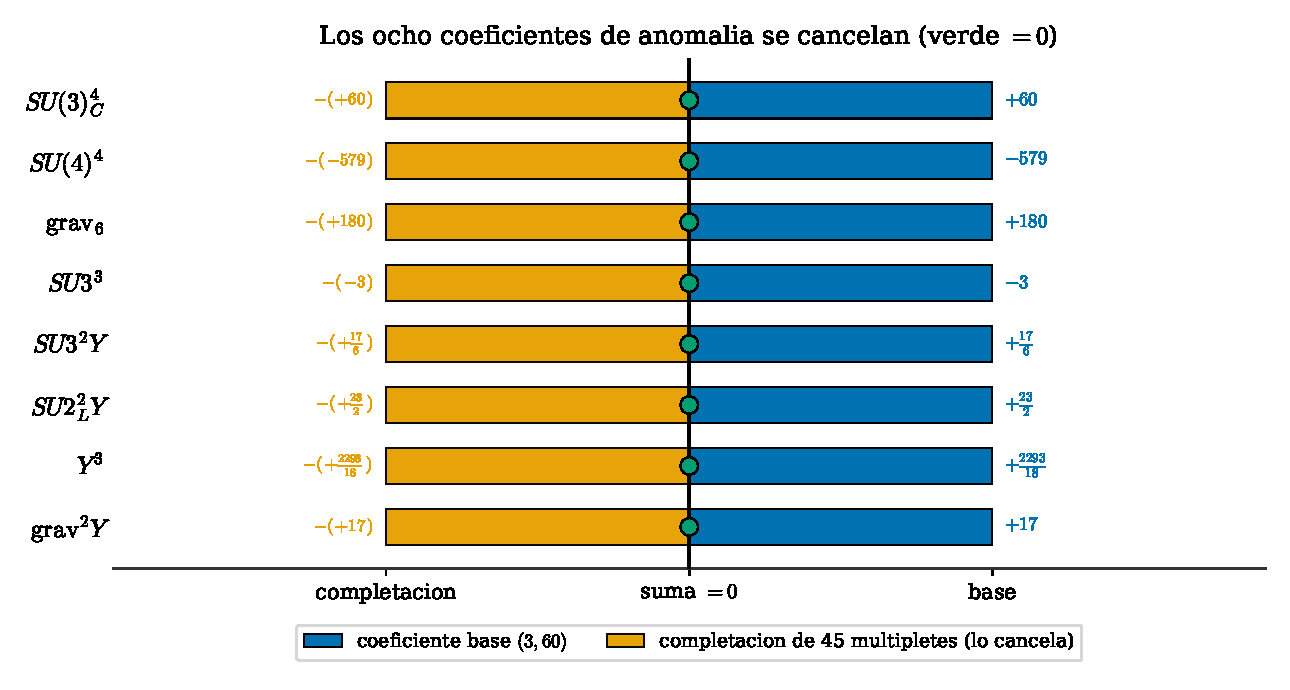
\includegraphics[width=0.82\linewidth]{fig_anomaly_cancel_es.pdf}
\caption{Los ocho coeficientes de anomal\'ia de bulk y de modo cero cuatridimensional del
bloque base $(3,\mathbf{60})$ (derecha, azul) y la contribuci\'on exactamente opuesta de la
completaci\'on de $45$ multipletes (izquierda, naranja); cada par suma cero (verde). Los
coeficientes son racionales exactos, recalculados independientemente.}
\label{fig:anomcancel}
\end{figure}

\begin{figure}[t]
\centering
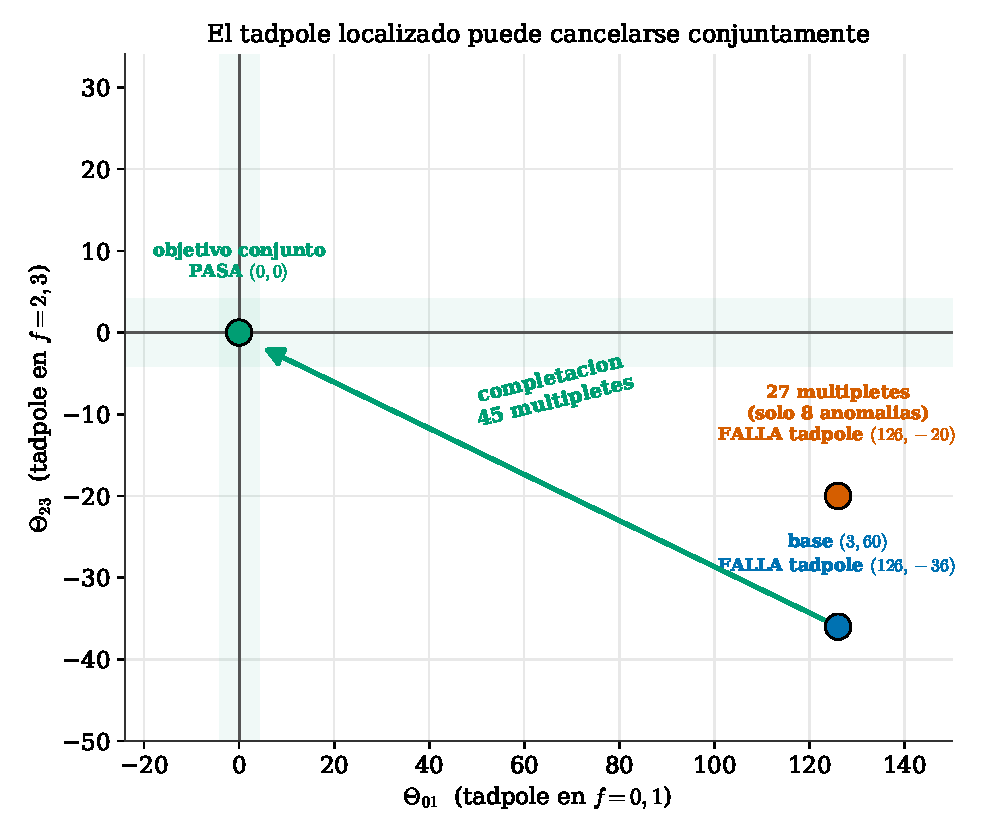
\includegraphics[width=0.80\linewidth]{fig_tadpole_journey_es.pdf}
\caption{El plano del tadpole localizado $(\Theta_{01},\Theta_{23})$. El bloque base se
sit\'ua en $\Theta_{\rm base}=(126,-36)$ y \emph{falla} el tadpole; el testigo de ocho
anomal\'ias de $27$ multipletes s\'olo llega a $(126,-20)$ y sigue fallando; la
completaci\'on de $45$ multipletes (flecha verde) lleva el total al origen. La libertad de
anomal\'ias por s\'i sola no cancela el tadpole --- pero una completaci\'on conjunta s\'i.}
\label{fig:tadmap}
\end{figure}

\begin{figure}[t]
\centering
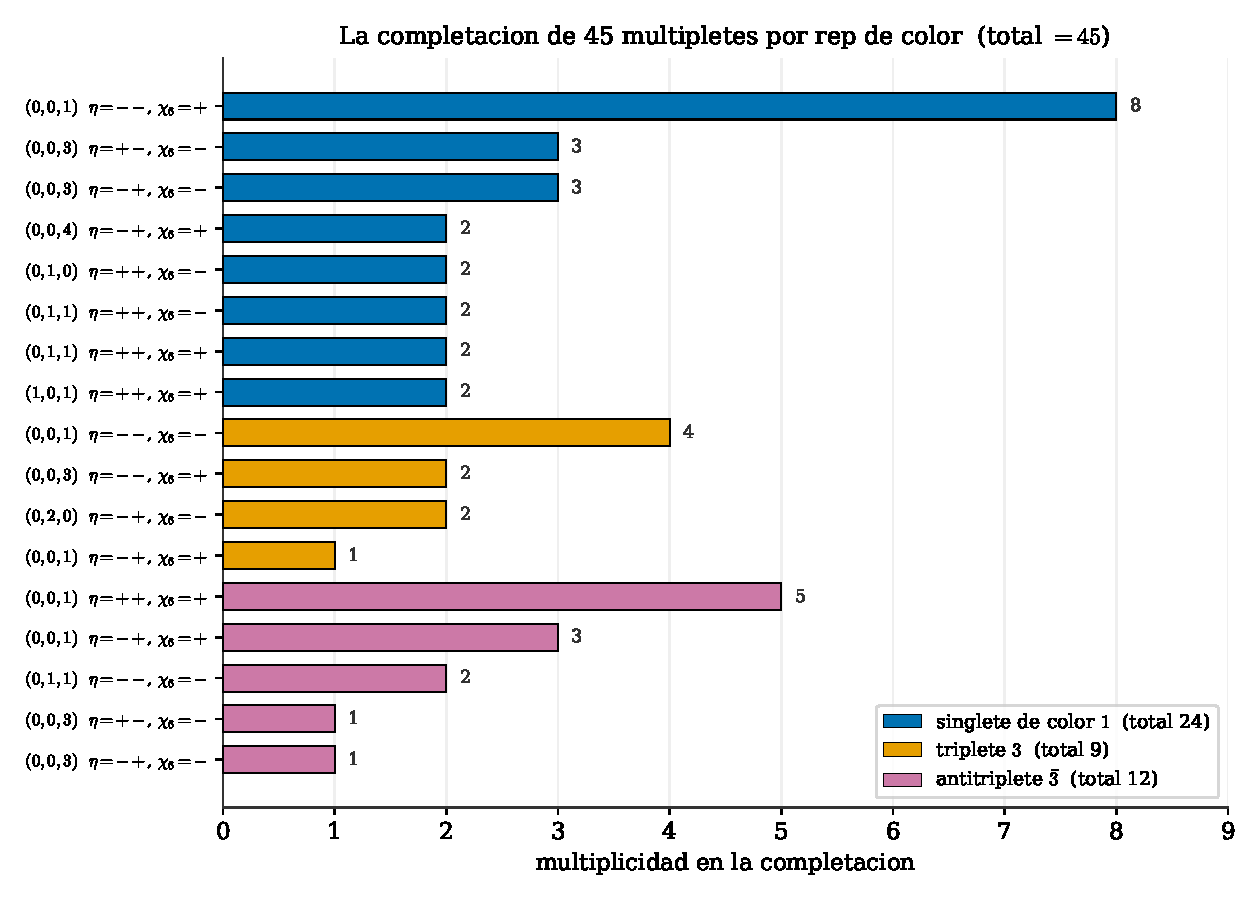
\includegraphics[width=0.86\linewidth]{fig_spectrum45_es.pdf}
\caption{La completaci\'on de $45$ multipletes, agrupada por representaci\'on de color
(etiqueta de Dynkin, paridad intr\'inseca $\eta$, quiralidad de seis dimensiones $\chi_6$;
las multiplicidades suman $45$). \textbf{Verificado: ocho anomal\'ias $+$ tadpole localizado
$+$ integralidad c\'ubica local; la condici\'on de masa ($\S\ref{sec:n7}$) pendiente.}}
\label{fig:witness45}
\end{figure}

\begin{table}[t]
\centering\small
\rowcolors{2}{softgrey}{white}
\begin{tabular}{clcccc}
\toprule
\rowcolor{hdrblue}
\textcolor{white}{\#} & \textcolor{white}{Dynkin $(a,b,c)$} & \textcolor{white}{color} &
\textcolor{white}{$\eta=(p_0,p_2)$} & \textcolor{white}{$\chi_6$} & \textcolor{white}{mult.}\\
\midrule
1  & $(0,0,1)$ & $\mathbf{1}$ & $(-,-)$ & $+$ & 8\\
2  & $(0,0,3)$ & $\mathbf{1}$ & $(+,-)$ & $-$ & 3\\
3  & $(0,0,3)$ & $\mathbf{1}$ & $(-,+)$ & $-$ & 3\\
4  & $(0,0,4)$ & $\mathbf{1}$ & $(-,+)$ & $+$ & 2\\
5  & $(0,1,0)$ & $\mathbf{1}$ & $(+,+)$ & $-$ & 2\\
6  & $(0,1,1)$ & $\mathbf{1}$ & $(+,+)$ & $-$ & 2\\
7  & $(0,1,1)$ & $\mathbf{1}$ & $(+,+)$ & $+$ & 2\\
8  & $(1,0,1)$ & $\mathbf{1}$ & $(+,+)$ & $+$ & 2\\
\rowcolor{white}\multicolumn{5}{r}{\textit{subtotal singletes de color}} & \textit{24}\\
9  & $(0,0,1)$ & $\mathbf{3}$ & $(-,+)$ & $+$ & 1\\
10 & $(0,0,1)$ & $\mathbf{3}$ & $(-,-)$ & $-$ & 4\\
11 & $(0,0,3)$ & $\mathbf{3}$ & $(-,-)$ & $+$ & 2\\
12 & $(0,2,0)$ & $\mathbf{3}$ & $(-,+)$ & $-$ & 2\\
\rowcolor{white}\multicolumn{5}{r}{\textit{subtotal tripletes}} & \textit{9}\\
13 & $(0,0,1)$ & $\bar{\mathbf{3}}$ & $(+,+)$ & $+$ & 5\\
14 & $(0,0,1)$ & $\bar{\mathbf{3}}$ & $(-,+)$ & $+$ & 3\\
15 & $(0,0,3)$ & $\bar{\mathbf{3}}$ & $(+,-)$ & $-$ & 1\\
16 & $(0,0,3)$ & $\bar{\mathbf{3}}$ & $(-,+)$ & $-$ & 1\\
17 & $(0,1,1)$ & $\bar{\mathbf{3}}$ & $(-,-)$ & $-$ & 2\\
\rowcolor{white}\multicolumn{5}{r}{\textit{subtotal antitripletes}} & \textit{12}\\
\midrule
\rowcolor{hdrblue}\multicolumn{5}{r}{\textcolor{white}{\textbf{total}}} & \textcolor{white}{\textbf{45}}\\
\bottomrule
\end{tabular}
\caption{La completaci\'on completa de $45$ multipletes: las $17$ especies por etiqueta de
Dynkin $(a,b,c)$ de $SU(4)$, representaci\'on de color, paridad intr\'inseca
$\eta=(p_0,p_2)$, quiralidad de seis dimensiones $\chi_6$ y multiplicidad. Es el espectro
que cancela los ocho coeficientes de anomal\'ia y el tadpole localizado con residuos
c\'ubicos locales enteros (\S\ref{sec:witness}); reverificado de forma independiente en
aritm\'etica racional exacta por \texttt{r60\_verify\_joint.sage}.}
\label{tab:spectrum}
\end{table}

% ===================================================================
\section{De un testigo a una garant\'ia: el tadpole nunca obstruye}\label{sec:existence}
Todo constructor de modelos conoce la duda callada que sigue a un hallazgo afortunado:
¿era una ley, o solo esta vez? El espectro de $45$ multipletes de la secci\'on anterior
cancela las anomal\'ias y el tadpole a la vez --- pero un ejemplo es una coincidencia
hasta que se demuestra lo contrario, y todo el temple de este art\'iculo es preferir un
certificado a una coincidencia. As\'i que apretamos la pregunta m\'as aguda que el testigo
no puede responder por s\'i solo: ¿es la cancelaci\'on conjunta \emph{inevitable}, o
$(3,\mathbf{60})$ simplemente tuvo suerte? La respuesta, resulta, no necesita m\'as
b\'usqueda --- solo dos hechos elementales, porque las anomal\'ias y el tadpole son ambos
funcionales \emph{lineales} de las multiplicidades a\~nadidas. Escribimos $A$ para el mapa
de anomal\'ias (a $\mathbb{Q}^8$) y $\Theta$ para el del tadpole localizado (a
$\mathbb{Q}^2$) sobre la biblioteca de adiciones. Dos preguntas deciden entonces todo.
Primera: ¿son el tadpole y las anomal\'ias mandos \emph{independientes}, o hay una
combinaci\'on oculta $\varphi\circ\Theta$ que queda fija una vez canceladas las
anomal\'ias --- una ley de conservaci\'on que clavar\'ia el tadpole lejos de cero?
Segunda: como solo se puede \emph{a\~nadir} materia, nunca restar, ¿pueden las adiciones
que dejan intactas las ocho anomal\'ias empujar a\'un el tadpole en \emph{toda}
direcci\'on? Ambas respuestas resultan favorables, y exactamente.

Volvamos ahora a la pregunta que qued\'o abierta en la introducci\'on --- la que Scrucca,
Serone, Silvestrini y Wulzer plantearon en 2003. Dos d\'ecadas estuvo seca: todos coincid\'ian
en que un modelo realista necesitaba un espectro anomal\'ia-libre con tadpole globalmente
nulo, todos sab\'ian que las dos condiciones eran independientes y, aun as\'i, la soluci\'on
conjunta se trataba como una esperanza modelo a modelo --- algo con lo que tropezar, no algo
garantizado. Las dos preguntas de arriba acaban con esa sequ\'ia. La primera, la
independencia, ya era observaci\'on suya; lo nuestro es hacerla \emph{exacta} --- un
certificado de determinante de rango pleno sobre toda la biblioteca, no una nota al paso. La
segunda es la genuinamente nueva, y su respuesta es el giro de la historia: la materia
anomal\'ia-neutra alcanza \emph{cualquier} valor del tadpole. Ese solo hecho convierte la
independencia en una \emph{garant\'ia} de no-obstrucci\'on, y zanja el requisito de veintid\'os
a\~nos --- no para un espectro afortunado, sino estructuralmente, para toda la clase a la vez.
Es nuestro resultado estructural principal.

¿Por qu\'e estuvo tanto tiempo en pie la pregunta? No por falta de esfuerzo --- el campo la
rond\'o durante dos d\'ecadas --- sino porque se hac\'ia en el idioma equivocado y se buscaba
en el lugar equivocado. La construcci\'on de modelos es, por vieja costumbre, una b\'usqueda:
se elige un contenido fermi\'onico, se pregunta si las anomal\'ias se cancelan \emph{y} el
tadpole se anula, y cuando no --- como casi siempre --- se elige otro y se vuelve a empezar. Es
una cinta de correr, y cada paso fallido susurra la misma sugerencia desalentadora, que quiz\'as
no exista paso alguno; la nota final de SSSW arrastra exactamente esa fatiga. Y los caminos que
el campo \emph{s\'i} tom\'o llevaban a otra parte. Una tradici\'on busc\'o \emph{prohibir} el
tadpole de ra\'iz, disponiendo una simetr\'ia bajo la cual no puede surgir --- la
``unificaci\'on gauge-Higgs sin tadpoles'' de Biggio y Quir\'os~\cite{BiggioQ} ---, una salida
genuina, pero disponible solo en configuraciones especiales, y de ninguna ayuda para cancelar un
tadpole que ya est\'a ah\'i. Otra se apoy\'o en el reflejo m\'as antiguo frente a las
anomal\'ias: a\~nadir materia \emph{vector-like}, que las mata gratis. Pero el tadpole localizado
es ciego a la quiralidad, de modo que un par vector-like lo \emph{dobla} en vez de aliviarlo ---
el instrumento m\'as familiar en la mano del constructor de modelos es, aqu\'i, justo el
equivocado. Lo que el problema ped\'ia en voz baja era el gesto contrario: a\~nadir materia
\emph{quiral}, cada especie an\'omala por s\'i sola pero sumando cero, y en cantidad suficiente
para conducir el tadpole a casa --- algo antinatural de intentar a mano, y antinatural de desear
para un minimalista. La independencia, adem\'as, lo mismo que SSSW hab\'ian notado, es aqu\'i un
falso amanecer: saber que los dos diales giran
por separado no promete que ambos puedan ponerse a cero a la vez, porque al constructor de
modelos solo se le permite \emph{a\~nadir} materia, nunca quitarla. El objeto verdadero no es,
pues, un par de n\'umeros independientes, sino un \emph{cono} --- el conjunto de tadpoles
alcanzables amontonando materia anomal\'ia-neutra --- y un cono puede ser sesgado, abrirse hacia
un horizonte y quedar tapiado hacia otro. Nadie hab\'ia dibujado ese cono. Dos instintos lo
mantuvieron a oscuras. El primero es de vocabulario: la existencia de \emph{alguna}
completaci\'on, entre todas, es una pregunta de factibilidad --- de rangos, ret\'iculos enteros,
certificados de Farkas --- y esas son las herramientas de la optimizaci\'on combinatoria, un
pa\'is vecino que el constructor de modelos rara vez visita, de modo que la pregunta casi nunca
se plante\'o en una forma que pudiera zanjarse de una vez por todas. El segundo es de gusto, y el
m\'as humano de los dos: la completaci\'on que funciona no es escueta sino pr\'odiga ---
cuarenta y cinco multipletes vertidos --- y una disciplina educada para admirar la econom\'ia no
va a cavar donde la respuesta pesa. La soluci\'on estaba a la vista, en la \'unica direcci\'on
que la est\'etica hab\'ia dicho a todos que no miraran. C\'ambiese la b\'usqueda por un test de
factibilidad, dej\'ese a un lado el reflejo por la minimalidad, ll\'evense las herramientas del
optimizador --- y el muro de veintid\'os a\~nos se adelgaza hasta desaparecer: un rango, y un
cono.

\begin{theorem}[Existencia]\label{thm:existence}
Sobre la biblioteca de $SU(4)$ (dimensi\'on $\le35$, todos los colores, paridades y
quiralidades de seis dimensiones), el mapa combinado $(A,\Theta)$ tiene rango pleno
$10=8+2$, y la imagen de $\Theta$ sobre el cono anomal\'ia-neutro no-negativo
$\{x\ge0:Ax=0\}$ es todo $\mathbb{R}^2$. En consecuencia, el tadpole localizado no impone
\emph{ninguna} obstrucci\'on m\'as all\'a de la libertad de anomal\'ias: toda
completaci\'on anomal\'ia-libre de $(3,\mathbf{60})$ admite una tadpole-compatible. El
espectro de $45$ multipletes es una realizaci\'on, representativa y no excepcional.
\end{theorem}

\noindent La demostraci\'on son dos certificados exactos. \emph{Independencia:} el mapa
apilado $[A;\Theta]$ tiene rango $10$ --- un menor entero $10\times10$ expl\'icito tiene
determinante $3.6\times10^{20}\neq0$ --- as\'i que las dos componentes del tadpole no son
ninguna combinaci\'on de los ocho coeficientes de anomal\'ia y ning\'un invariante
$\varphi\circ\Theta$ se conserva. (Si el rango fuera deficiente, tal combinaci\'on
conservada existir\'ia; el espectro anomal\'ia-libre de $27$ multipletes, que a\'un porta
tadpole $(126,-20)\neq0$, ya muestra que el tadpole genuinamente no queda fijado por las
anomal\'ias.) \emph{Alcanzabilidad:} adiciones anomal\'ia-neutras no-negativas realizan
cada eje del tadpole con signo --- $\Theta=(288,0)$ por dos multipletes, $(0,48)$ por
cuatro, y sus negativos igual. Cuatro direcciones que generan positivamente el plano ponen
el $0$ en el interior del cono alcanzable, de modo que cualquier tadpole residual que porte
un embedding anomal\'ia-libre, la materia anomal\'ia-neutra lo cancela
(Figura~\ref{fig:cone}). Todo es \'algebra lineal racional exacta, y los cuatro testigos
junto con su independencia se reverifican en el n\'ucleo de Lean~4
(\texttt{R60JointExistence.lean}, dependiendo solo de \texttt{propext}). \hfill$\square$

\begin{figure}[t]
\centering
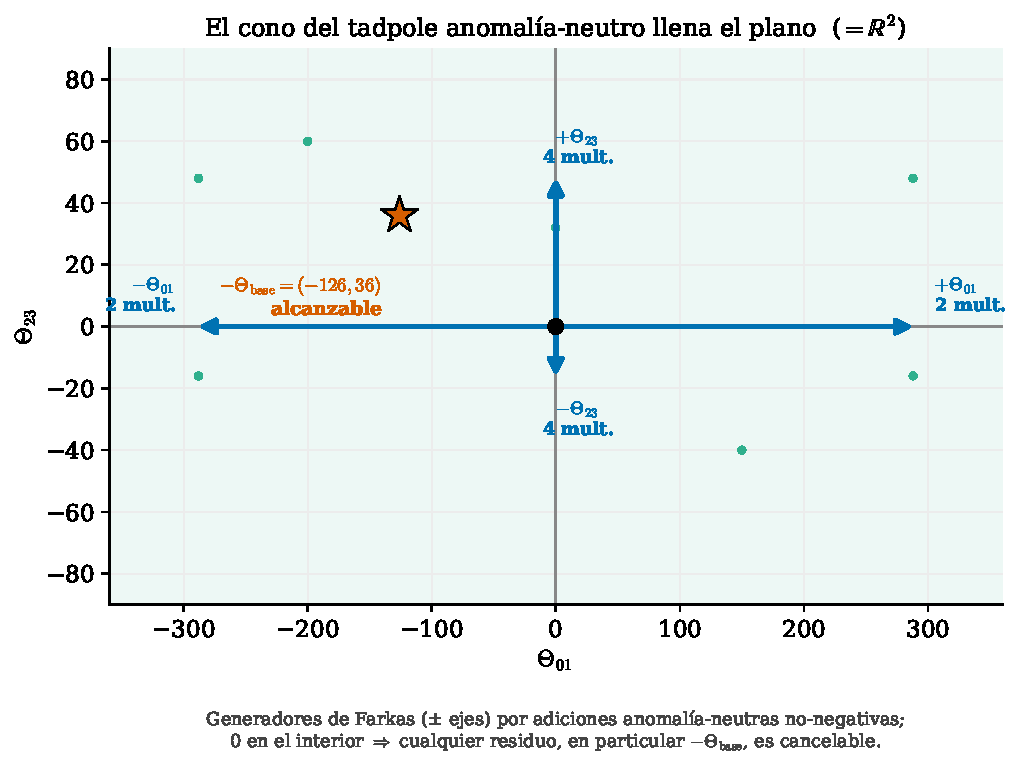
\includegraphics[width=0.70\linewidth]{fig_cone_es.pdf}
\caption{El Teorema~\ref{thm:existence}, en imagen. Adiciones anomal\'ia-neutras
no-negativas realizan ambos signos de cada eje del tadpole (flechas azules, etiquetadas
por el n\'umero de multipletes --- los certificados de Farkas), de modo que el cono que
generan es todo el plano $\mathbb{R}^2$ (sombreado). El origen es interior; luego el
residuo base $-\Theta_{\rm base}=(-126,36)$ (estrella) --- y cualquier otro --- es
cancelable a\~nadiendo materia anomal\'ia-neutra.}
\label{fig:cone}
\end{figure}

Tras el \'algebra lineal hay una imagen que vale la pena guardar. El tadpole es una
cantidad \emph{blanda} --- una suma con signo, pesada por paridad, cuyo signo se voltea con
la paridad intr\'inseca y la quiralidad de seis dimensiones de la materia que se a\~nade ---
mientras que los polinomios de anomal\'ia son r\'igidos. El cat\'alogo fermi\'onico es, por
tanto, lo bastante rico para \emph{orientar} el tadpole a donde uno quiera, en cualquier
direcci\'on, sin mover un solo coeficiente de anomal\'ia. Le\'ido as\'i, el espectro de
$45$ multipletes nunca fue una aguja en un pajar: el pajar est\'a hecho de agujas, y
simplemente recogimos una.

Y el m\'etodo sobrevive al ejemplo. Su forma es independiente del modelo: para
\emph{cualquier} biblioteca fermi\'onica de orbifold, el mismo test de
\textbf{rango\,$+$\,cono} decide si un funcional localizado es una obstrucci\'on
independiente (un invariante conservado, o un cono puntiagudo --- un no-go inmediato cuando
la base lo viola) o es siempre absorbible. Lo publicamos como la herramienta anexa
\texttt{ghu\_preflight.py}: dada una biblioteca fermi\'onica (representaciones, colores,
paridades, quiralidades) y un bloque base, devuelve el veredicto exacto ---
\textsc{unobstructed}, \textsc{no-go} o \textsc{cone-obstructed} --- con su certificado de
rango/Farkas, con el modelo f\'isico como un \'unico callback intercambiable. Por modelo se
obtiene un veredicto decisivo; si obstruido, el invariante conservado expl\'icito
$\varphi\circ\Theta$ (una firma candidata de baja energ\'ia); si no-obstruido, la
garant\'ia de que una b\'usqueda entera termina con \'exito junto con las direcciones
constructivas de Farkas para \emph{construir} una completaci\'on sin solucionador; y,
corri\'endolo sobre una familia de embeddings, una clasificaci\'on del landscape en
obstruidos y no-obstruidos. Es, pues, un preflight exacto antes de una b\'usqueda cara ---
decisi\'on-completo por ambos lados --- y una forma de cazar los modelos genuinamente
obstruidos, donde la libertad de anomal\'ias no implica la del tadpole.

Con esto, el acto central de la historia se cierra, y limpiamente: el bloque
$(3,\mathbf{60})$ es \emph{consistente}, y de forma demostrable --- por una ley, no un
ejemplo. \emph{Establecido:} la cancelaci\'on del tadpole no es obstrucci\'on m\'as all\'a
de la libertad de anomal\'ias; toda completaci\'on anomal\'ia-libre admite una.
\emph{Queda abierto:} el enunciado entero plenamente general sobre todos los embeddings (un
check finito de base de Hilbert --- el cono racional ya es todo el plano). Lo que no se sabe
a\'un del bloque es que sea \emph{viable}; y para eso resta la \'ultima y m\'as estricta
pregunta del viaje.

% ===================================================================
\section{El filtro de masa de frontera y el veredicto f\'isico}\label{sec:n7}
Una completaci\'on consistente con anomal\'ias y tadpole a\'un porta modos cero ex\'oticos.
Las masas de frontera pueden emparejarlos, pero la pregunta aguda es si pueden hacerlo
dejando $Q$, $u_R$, $d_R$ sin masa. Una masa de Dirac localizada en un punto fijo empareja
un modo cero del bulk con un fermi\'on de Weyl de brana de representaci\'on local conjugada
y quiralidad cuatridimensional opuesta; si \emph{todos} los ex\'oticos pueden levantarse
as\'i mientras cada objetivo permanece en el n\'ucleo es exactamente una condici\'on de
emparejamiento bipartito (de rango gen\'erico) sobre el grafo de masas permitidas. Es una
prueba finita y exacta --- termina con un veredicto definido, no con un tiempo agotado --- y
hemos validado el solucionador en casos de respuesta conocida. Dos hechos estructurales la
agudizan: los modos cero ex\'oticos zurdos y diestros portan representaciones de $SU(2)_L$
que no casan, de modo que los compa\~neros de brana son inevitables; y la multiplicidad dos
de $Q_L$ obliga a levantar un doblete degenerado protegiendo a su gemelo, una deficiencia de
rango posible pero no autom\'atica.

Ejecutar esta condici\'on frente a la biblioteca de brana completa en las dos clases de
punto fijo, e imponer la paridad global de $SU(2)$ que proh\'ibe un n\'umero impar de
dobletes de Weyl (la anomal\'ia de Witten~\cite{Witten82}), es el paso f\'isico decisivo. Lo
reportamos como abierto: el veredicto determina si la completaci\'on $(3,\mathbf{60})$ es
viable --- un sector de quarks realista del modelo de dos dobletes de Higgs de AHMN --- o un
no-go, en cuyo caso la obstrucci\'on porta una firma concreta de baja energ\'ia (ex\'oticos
ligeros inevitables o un compa\~nero vector-like de un quark del Modelo Est\'andar). Cualquier
desenlace es un resultado de la jerarqu\'ia exacta; ninguno se reclama aqu\'i.

% ===================================================================
\section{Firmas de baja energ\'ia de los dos veredictos}\label{sec:signatures}
Conc\'edase a la jerarqu\'ia exacta sus dos respuestas posibles --- ¿c\'omo se ver\'ia cada
una en un experimento? El valor de fijar la pregunta de consistencia es que los dos
desenlaces no son fenomenol\'ogicamente intercambiables: cada uno se corresponde con una
firma de baja energ\'ia distinta y, en principio, falsable. Una predicci\'on robusta
sobrevive de cualquier modo. Como la construcci\'on de AHMN subyacente entrega \emph{dos}
dobletes de Higgs como modos cero de l\'inea de Wilson~\cite{AHMN}, el sector escalar es el
de un modelo de dos dobletes de Higgs, con los estados extra $H$, $A$, $H^\pm$ que le
acompa\~nan y las cuestiones de alineamiento de sabor que tales modelos
cargan~\cite{2HDM}; en la unificaci\'on gauge--Higgs su potencial es radiativo y finito, de
modo que las masas y mezclas de los dobletes est\'an ligadas a la din\'amica de
compactificaci\'on en vez de ser libres~\cite{Hosotani}. Nuestro an\'alisis no calcula esas
masas, pero fija el escenario en el que viven.

Si el filtro de masa de frontera \emph{pasa} --- todo ex\'otico levantado a la escala de
compactificaci\'on $1/R$ mientras $Q,u_R,d_R$ permanecen sin masa --- la teor\'ia ligera es
el Modelo Est\'andar m\'as ese segundo doblete, y la huella distintiva de alta escala es una
torre de excitaciones de Kaluza--Klein de los campos gauge y de materia en $1/R$, la
firma gen\'erica de las dimensiones extra. Si en cambio el filtro devuelve un \emph{no-go},
la obstrucci\'on no es abstracta: la deficiencia de rango del emparejamiento deja un remanente
f\'isico. Son posibles dos formas. O bien un modo cero ex\'otico no puede emparejarse en
absoluto y sobrevive como un estado ligero inevitable --- una part\'icula coloreada o con
carga d\'ebil cerca de la ventana electrod\'ebil--TeV, el falsador m\'as agudo posible --- o
bien el \'unico modo de levantar el doblete ex\'otico es emparejarlo con un compa\~nero que
tambi\'en despose a un quark del Modelo Est\'andar, dejando un \emph{quark vector-like}: un
compa\~nero no quiral de $Q$, $u_R$ o $d_R$ que se mezcla con las generaciones ligeras y se
busca directamente en colisionadores mediante producci\'on simple y en pares~\cite{VLQ}. La
multiplicidad dos de $Q_L$ aislada en \S\ref{sec:hypercharge} es exactamente lo que hace
natural esta segunda opci\'on --- dos dobletes de cargas id\'enticas, uno de los cuales debe
recibir una masa vector-like --- de modo que un compa\~nero vector-like de $Q$ es la firma
espec\'ifica que un no-go aqu\'i portar\'ia.

¿Cu\'an pesados, y c\'omo se distinguir\'ian? La unificaci\'on gauge--Higgs liga la escala de
compactificaci\'on $1/R$ a la masa del Higgs generada radiativamente; reproducir
$m_h=125$~GeV con un potencial de Coleman--Weinberg dominado por el top empuja t\'ipicamente
$1/R$ al rango multi-TeV, de modo que la torre de Kaluza--Klein y los escalares m\'as pesados
del sector de dos dobletes se situar\'ian ah\'i, en o m\'as all\'a del alcance actual de los
colisionadores. Un quark vector-like no tiene por qu\'e, sin embargo, vivir en $1/R$: si surge
de una deficiencia de rango de masa de frontera, su masa es un par\'ametro de brana y podr\'ia
ser considerablemente m\'as ligera, al alcance del LHC y su fase de alta luminosidad. Tal
estado se anunciar\'ia en los canales establecidos de quarks vector-like~\cite{VLQ} ---
producci\'on en pares seguida de desintegraciones a $Wq$, $Zq$ o $hq$, o producci\'on simple
por su mezcla con las generaciones ligeras --- y la multiplicidad dos de $Q_L$ apunta
espec\'ificamente a un compa\~nero en el sector del doblete $(t,b)$. La otra rama de no-go, un
ex\'otico que no puede emparejarse en absoluto, aflorar\'ia en cambio como un estado coloreado
o con carga d\'ebil estable o de vida larga cerca de la escala electrod\'ebil, una se\~nal m\'as
aguda y m\'as inmediatamente falsable. La distinci\'on no es, por tanto, acad\'emica: un
veredicto sit\'ua la nueva f\'isica en $1/R$ muy arriba, el otro un quark vector-like
posiblemente ya al alcance. Ninguna de estas masas se calcula aqu\'i --- est\'an aguas abajo
del filtro de masa y de los datos de compactificaci\'on --- pero las \emph{clases} de se\~nal
quedan fijadas por la estructura establecida arriba.

\emph{Establecido:} caiga como caiga el veredicto, el marco predice robustamente un segundo
doblete de Higgs, y los dos veredictos se separan limpiamente en un espectro Kaluza--Klein/2HDM
por un lado y una firma de ex\'otico ligero o quark vector-like por el otro. \emph{Queda
abierto:} cu\'al de estos realiza el modelo, y la escala $1/R$ que fija las masas --- ninguna
calculada aqu\'i, ambas aguas abajo del filtro de masa.

% ===================================================================
\section{Consistencia, viabilidad, y qu\'e compra una respuesta exacta}\label{sec:reflection}
¿Qu\'e ense\~na este ejercicio concreto sobre la brecha entre una teor\'ia consistente y una
viable? El caso agudiza una distinci\'on f\'acil de difuminar. La \emph{consistencia} ---
libertad de anomal\'ias, cancelaci\'on de tadpole --- es una afirmaci\'on sobre el
ultravioleta; la \emph{viabilidad} --- un espectro ligero que es el Modelo Est\'andar y nada
m\'as --- es una afirmaci\'on sobre el infrarrojo. La unificaci\'on gauge--Higgs hace visible
la costura: el Higgs es una l\'inea de Wilson, de modo que los mismos datos de orbifold que
fijan las anomal\'ias moldean tambi\'en el potencial del Higgs, y sin embargo la obstrucci\'on
de anomal\'ia es topol\'ogica y ciega al vac\'io del Higgs, mientras que la masa de los
ex\'oticos es una cuesti\'on espectral, infrarroja. Un modelo puede ser perfectamente
consistente y a\'un fallar en ser viable, y s\'olo un filtro infrarrojo --- aqu\'i el
emparejamiento de masa de frontera --- lo decide.

Hay una reflexi\'on sobre el propio Higgs, y sobre por qu\'e sigue tan dif\'icil de fijar. En
la unificaci\'on gauge--Higgs las mismas componentes internas $A_5,A_6$ son a la vez campo
gauge y Higgs; cu\'al de las dos muestra la teor\'ia depende del vac\'io en que se asienta, de
modo que el Higgs no tiene identidad fija independiente de la l\'inea de Wilson que cabalga. Esa
elusividad no es un incordio sino la fuente de su buen comportamiento --- un objeto sin
definici\'on local no admite contrat\'ermino de masa local --- y es exactamente lo que el
tadpole localizado amenaza con estropear, alimentando un t\'ermino de punto fijo directamente
a una masa que el mecanismo fue construido para proteger. Le\'ida as\'i, toda la jerarqu\'ia de
consistencia es un conjunto de condiciones para mantener al Higgs esquivo: la libertad de
anomal\'ias y la cancelaci\'on del tadpole son el precio de un escalar protegido precisamente
porque nunca es del todo un escalar. La completaci\'on que exhibimos paga ese precio a nivel de
orbifold; si el infrarrojo entrega entonces un Higgs del Modelo Est\'andar y nada m\'as es la
pregunta que sostiene el filtro de masa.

Hay tambi\'en una reflexi\'on metodol\'ogica. ¿D\'onde, cuando la aritm\'etica est\'a
verificada por m\'aquina, vive la \'ultima libertad de equivocarse? No en los n\'umeros --- en
la frase que los nombra. Cuando cada eslab\'on del argumento es un certificado verificable por
m\'aquina, el modo de fallo de la construcci\'on de modelos se desplaza: el peligro ya no es un
desliz aritm\'etico sino una \emph{mala interpretaci\'on} --- un n\'umero cierto pegado a una
frase falsa. Hacer el flujo exacto no elimina ese peligro, pero lo a\'isla, y deja que un giro
equivocado sea atrapado por la verdad de referencia y no por el gusto. Varias afirmaciones
intermedias plausibles en este mismo estudio fueron refutadas as\'i antes de entrar en el
art\'iculo --- una normalizaci\'on por factor dos en la hipercarga, y una propuesta de
correcci\'on vector-like del tadpole que el ret\'iculo entero descart\'o. En ese sentido la
contribuci\'on es tanto sobre \emph{c\'omo} pueden zanjarse tales preguntas como sobre la
respuesta particular para $(3,\mathbf{60})$.

% ===================================================================
\section{Metodolog\'ia y reproducibilidad}\label{sec:method}
Toda afirmaci\'on de arriba es un c\'alculo exacto y finito. Los coeficientes de anomal\'ia y
tadpole son sumas racionales exactas sobre pesos de $SU(4)$ (SageMath); la factibilidad
acoplada se estudia con ramificaci\'on y acotaci\'on exacta (PPL), OR-Tools CP-SAT y
certificados de ret\'iculo por capas (forma normal de Smith), con el testigo de $45$
multipletes reverificado en racionales exactos; la condici\'on de masa de frontera es
emparejamiento bipartito exacto; y el fragmento de c\'ubicas localizadas est\'a certificado sin
axiomas en Lean~4. Somos expl\'icitos sobre lo que \emph{no} se establece: la b\'usqueda acotada
general es \texttt{UNKNOWN}, y no se produjo un certificado de base de Hilbert (Normaliz) a esta
dimensi\'on. El material anexo contiene los scripts, el espectro completo de $45$ multipletes, la
tabla de restricciones con el estado y alcance de cada condici\'on, y la fuente Lean, de modo que
cada n\'umero aqu\'i pueda regenerarse. Los c\'alculos exactos se realizaron y se contrastaron
por dos agentes independientes trabajando frente a esta verdad de referencia com\'un; ese
m\'etodo de trabajo, m\'as que ning\'un n\'umero aislado, es lo que m\'as redujo los errores de
interpretaci\'on a los que es propenso un an\'alisis de construcci\'on de modelos.

La Tabla~\ref{tab:artifacts} lista los artefactos verificables por m\'aquina publicados con este
art\'iculo; cada entrada regenera una afirmaci\'on espec\'ifica de arriba.

\begin{table}[h]
\centering
\footnotesize
\rowcolors{2}{softgrey}{white}
\begin{tabular}{lll}
\toprule
\rowcolor{hdrblue}
\textcolor{white}{Artefacto} & \textcolor{white}{Certifica} & \textcolor{white}{Herramienta}\\
\midrule
\texttt{R60LocalizedAnomaly.lean} & residuos c\'ubicos locales, $\dim=60$, dependencia de Wilson & Lean~4 (sin axiomas)\\
\texttt{R60JointExistence.lean}   & certificado cono/independencia del Teorema de Existencia & Lean~4 (solo \texttt{propext})\\
\texttt{r60\_sm\_embedding.sage}   & hipercarga $Y=(-7q_8+4q_{15})/18$; cargas ME & SageMath (exacto)\\
\texttt{r60\_anomalies.sage}       & ocho coeficientes bulk/modo cero de $(3,\mathbf{60})$ & SageMath (exacto)\\
\texttt{r60\_tadpole.sage}         & tadpole localizado $\Theta_{\rm base}=(126,-36)$ & SageMath (exacto)\\
\texttt{r60\_cpsat.sage}           & la b\'usqueda de completaci\'on conjunta de $45$ multipletes & OR-Tools CP-SAT\\
\texttt{r60\_verify\_joint.sage}   & reverificaci\'on independiente del testigo de $45$ multipletes & SageMath (exacto)\\
\texttt{r60\_n7\_matching.sage}    & condici\'on bipartita de masa de frontera (casos validados) & OR-Tools / exacto\\
\texttt{structural\_theorem.sage} & $\operatorname{rank}[A;\Theta]=10$ y el cono del tadpole (Teor.~\ref{thm:existence}) & SageMath (exacto)\\
\texttt{ghu\_preflight.py}        & or\'aculo reutilizable rango$+$cono de obstrucci\'on (cualquier modelo) & SageMath (exacto)\\
\texttt{make\_paper\_graphics.py}  & Figuras~\ref{fig:anomcancel}--\ref{fig:witness45} a partir de los datos verificados & Matplotlib\\
\bottomrule
\end{tabular}
\caption{Manifiesto de reproducibilidad. Cada artefacto regenera una afirmaci\'on del
art\'iculo; el fichero Lean lo verifica el n\'ucleo sin axiomas m\'as all\'a de los propios de
Lean y sin \texttt{sorry}. Publicado con el material anexo.}
\label{tab:artifacts}
\end{table}

% ===================================================================
\section{Conclusi\'on}\label{sec:conclusion}
La lecci\'on principal es concreta, y cierra una pregunta m\'as vieja que el propio modelo. La
libertad de anomal\'ias y la cancelaci\'on del tadpole localizado --- llamadas condiciones
\emph{independientes} por Scrucca, Serone, Silvestrini y Wulzer en 2003, que dejaron la
construcci\'on de un espectro anomal\'ia-libre con tadpole globalmente nulo como problema abierto
--- no son aqu\'i meramente compatibles: se prueba que el tadpole \emph{nunca} obstruye una
completaci\'on anomal\'ia-libre, de modo que, tras dos d\'ecadas, su requisito se cumple no por
suerte sino como garant\'ia estructural, exacta y verificada por m\'aquina. El bloque
$(3,\mathbf{60})$, que un barrido muestra ser la representaci\'on m\'inima capaz de albergar los
quarks, lo realiza expl\'icitamente --- una completaci\'on de $45$ multipletes que cancela los
ocho coeficientes de anomal\'ia y el tadpole localizado \emph{juntos}, con residuos c\'ubicos
locales enteros y dos certificados verificados en Lean. Lo que resta es la pregunta m\'as aguda de
todas --- si ese espectro consistente es tambi\'en f\'isicamente viable, con sus ex\'oticos
levantados y s\'olo el Modelo Est\'andar ligero --- y es el filtro de masa de frontera, \'el
mismo una prueba exacta y finita, quien la decidir\'a. La consistencia, aqu\'i, se ha zanjado con
certificados; la viabilidad es el pr\'oximo certificado por ganar. Y la minimalidad de
$(3,\mathbf{60})$ hallada aqu\'i por barrido se convierte en una clasificaci\'on exacta de
\emph{qu\'e} representaciones de $SU(4)$ contienen la celda de quarks del Modelo Est\'andar en
el trabajo compa\~nero, la Parte~II~\cite{PartII}.

\appendix
% ===================================================================
\section{Convenciones de teor\'ia de grupos y los \'indices exactos}\label{app:conventions}
Para que cada n\'umero de arriba pueda regenerarse, fijamos aqu\'i las convenciones que codifican
los artefactos Lean y Sage. Un peso de $SU(4)$ se escribe por sus entradas de Young
$n_1\ge n_2\ge n_3\ge n_4$; las cargas internas usadas en todo el texto son
\begin{equation}
q_8=n_1+n_2-2n_3,\qquad q_{15}=n_1+n_2+n_3-3n_4,\qquad q_P=n_1+n_2-n_3-n_4,
\end{equation}
y las dos paridades de orbifold de un peso son $p_0=(-1)^{n_4}$, $p_2=(-1)^{n_3+n_4}$. La
hipercarga \eqref{eq:Y}, $Y=(-7q_8+4q_{15})/18$, es la \'unica combinaci\'on interna que asigna a
$Q_L,u_R,d_R$ sus cargas f\'isicas $1/6,2/3,-1/3$ (Tabla~\ref{tab:smcontent}) y preserva
$\sin^2\theta_W=\tfrac14$ a nivel \'arbol; los cuatro coeficientes de anomal\'ia dependientes de
$Y$ se dan en esta misma normalizaci\'on.

Las anomal\'ias de modo cero cuatridimensionales usan el \'indice de Dynkin del contenido de
esp\'in de $SU(2)_L$, $T_2(d)=\tfrac1{12}d(d^2-1)$ para una irrep de dimensi\'on $d$, ponderado
por la dimensi\'on de color y el signo de quiralidad de seis dimensiones; la c\'ubica pura
$SU(3)^3$ usa la normalizaci\'on c\'ubica fundamental. Los coeficientes de seis dimensiones usan
el \'indice cu\'artico $A_4$ de la irrep de $SU(4)$ (el coeficiente del $\Tr_4 F^4$ primitivo tras
restar la parte reducible $(\Tr F^2)^2$) y la dimensi\'on de la representaci\'on. Para el factor
de color $SU(3)$ no hay Casimir cu\'artico primitivo, de modo que $\Tr_3 F_C^4=\tfrac12(\Tr_3
F_C^2)^2$ y la entrada ``$SU(3)_C^4$'' es reducible; este es el origen de la forma cuadr\'atica de
rango dos de \S\ref{sec:bulkanom}. Los residuos c\'ubicos localizados en $f=0,1$ portan las
normalizaciones de punto fijo $\tfrac14$ (color) y $-\tfrac18$ ($SU(3)_{123}$), y las componentes
de tadpole son $\Theta_{01}\propto\sum \eta_0\,p_0\,q_{15}$ y $\Theta_{23}\propto\sum
\eta_2\,p_2\,q_P$ sobre los pesos, por la dimensi\'on de color.

Bajo $SU(3)_C\times[SU(3)_{123}\times U(1)_{15}]$ el bloque $(3,\mathbf{60})$ con $\eta=(+,+)$ se
descompone en los modos cero electrod\'ebiles de la Tabla~\ref{tab:smcontent} m\'as los ex\'oticos;
la completaci\'on de $45$ multipletes se lista por $(\text{Dynkin},\text{color},\eta,\chi_6)$ con
multiplicidades en su totalidad en la Tabla~\ref{tab:spectrum} y en el anexo
\texttt{r60\_verify\_joint.sage}. Todos los \'indices de este ap\'endice se recalculan exactamente
(sin coma flotante) por ese script y por \texttt{R60LocalizedAnomaly.lean}.

\begin{thebibliography}{99}
\bibitem{PartII} C.~Mar\'in, \emph{Three Gates to a Quark Generation: An Exact Criterion for
Which $SU(4)$ Representations Contain the Standard Model} (Parte~II), Zenodo (2026),
DOI:\,10.5281/zenodo.21432627.
% Todas las entradas arXiv/revista verificadas, 2026-07-18.
\bibitem{Manton} N.S.~Manton, \emph{A New Six-Dimensional Approach to the
Weinberg-Salam Model}, Nucl.\ Phys.\ B\textbf{158} (1979) 141.
\bibitem{Fairlie} D.B.~Fairlie, \emph{Higgs' fields and the determination of the
Weinberg angle}, Phys.\ Lett.\ B\textbf{82} (1979) 97.
\bibitem{Hosotani} Y.~Hosotani, \emph{Dynamical mass generation by compact extra
dimensions}, Phys.\ Lett.\ B\textbf{126} (1983) 309; Ann.\ Phys.\ \textbf{190} (1989) 233.
\bibitem{ColemanWeinberg} S.~Coleman, E.~Weinberg, \emph{Radiative Corrections as the
Origin of Spontaneous Symmetry Breaking}, Phys.\ Rev.\ D\textbf{7} (1973) 1888.
\bibitem{GreenSchwarz} M.B.~Green, J.H.~Schwarz, \emph{Anomaly Cancellation in
Supersymmetric $D=10$ Gauge Theory and Superstring Theory}, Phys.\ Lett.\ B\textbf{149}
(1984) 117.
\bibitem{Sagnotti} A.~Sagnotti, \emph{A note on the Green-Schwarz mechanism in
open-string theories}, Phys.\ Lett.\ B\textbf{294} (1992) 196, hep-th/9210127.
\bibitem{CallanHarvey} C.G.~Callan, J.A.~Harvey, \emph{Anomalies and Fermion Zero Modes
on Strings and Domain Walls}, Nucl.\ Phys.\ B\textbf{250} (1985) 427.
\bibitem{Witten82} E.~Witten, \emph{An $SU(2)$ Anomaly}, Phys.\ Lett.\ B\textbf{117}
(1982) 324.
\bibitem{KawamuraGUT} Y.~Kawamura, \emph{Triplet-doublet splitting, proton stability
and an extra dimension}, Prog.\ Theor.\ Phys.\ \textbf{105} (2001) 999, hep-ph/0103125.
\bibitem{ACG} N.~Arkani-Hamed, A.G.~Cohen, H.~Georgi, \emph{Anomalies on Orbifolds},
Phys.\ Lett.\ B\textbf{516} (2001) 395, hep-th/0103135.
\bibitem{GdVQ} G.~von Gersdorff, M.~Quir\'os, \emph{Localized anomalies in orbifold
gauge theories}, hep-th/0305024.
\bibitem{GdV6D} G.~von Gersdorff, \emph{Anomalies on Six Dimensional Orbifolds},
hep-th/0612212.
\bibitem{BiggioQ} C.~Biggio, M.~Quir\'os, \emph{Higgs-gauge unification without
tadpoles}, hep-ph/0407348.
\bibitem{SSSW} C.A.~Scrucca, M.~Serone, L.~Silvestrini, A.~Wulzer,
\emph{Gauge-Higgs Unification in Orbifold Models}, hep-th/0312267.
\bibitem{Kawamura} J.~Goto, Y.~Kawamura, T.~Miura, \emph{Orbifold Family Unification
on Six Dimensions}, arXiv:1307.2631.
\bibitem{aGUT} G.~Cacciapaglia, \emph{Systematic classification of aGUT models in five
dimensions: the $SU(N)$ kinship}, arXiv:2309.10098.
\bibitem{SU6GHGUT} A.~Angelescu, A.~Bally, F.~Goertz, S.~Weber, \emph{$SU(6)$
Gauge-Higgs Grand Unification: Minimal Viable Models and Flavor}, arXiv:2208.13782.
\bibitem{AHMN} K.~Akamatsu, T.~Hirose, N.~Maru, A.~Nago, \emph{Two Higgs Doublet Model
from Six Dimensional Gauge Theory}, arXiv:2603.05857.
\bibitem{2HDM} G.C.~Branco, P.M.~Ferreira, L.~Lavoura, M.N.~Rebelo, M.~Sher, J.P.~Silva,
\emph{Theory and phenomenology of two-Higgs-doublet models}, Phys.\ Rept.\ \textbf{516}
(2012) 1, arXiv:1106.0034.
\bibitem{VLQ} J.A.~Aguilar-Saavedra, R.~Benbrik, S.~Heinemeyer, M.~P\'erez-Victoria,
\emph{Handbook of vectorlike quarks: Mixing and single production}, Phys.\ Rev.\
D\textbf{88} (2013) 094010, arXiv:1306.0572.
\end{thebibliography}

\end{document}
